\section{Data Driven Background Estimation Methods}
\label{sec:datadriven}
We have developed two data-driven methods to 
estimate the background in the signal region.
The first one exploits the fact that 
SumJetPt and \met$/\sqrt{\rm SumJetPt}$ are nearly 
uncorrelated for the $t\bar{t}$ background 
(Section~\ref{sec:abcd});  the second one 
is based on the fact that in $t\bar{t}$ the
$P_T$ of the dilepton pair is on average 
nearly the same as the $P_T$ of the pair of neutrinos
from $W$-decays, which is reconstructed as \met in the
detector.


%{\color{red} I took these
%numbers from the twiki, rescaling from 11.06 to 30/pb.
%They seem too large...are they really right?}


\subsection{ABCD method}
\label{sec:abcd}

We find that in $t\bar{t}$ events SumJetPt and 
\met$/\sqrt{\rm SumJetPt}$ are nearly uncorrelated, 
as demonstrated in Fig.~\ref{fig:uncor}.
Thus, we can use an ABCD method in the \met$/\sqrt{\rm SumJetPt}$ vs
sumJetPt plane to estimate the background in a data driven way.

%\begin{figure}[bht]
%\begin{center}
%\includegraphics[width=0.75\linewidth]{uncorrelated.pdf}
%\caption{\label{fig:uncor}\protect Distributions of SumJetPt 
%in MC $t\bar{t}$ events for different intervals of 
%MET$/\sqrt{\rm SumJetPt}$.}
%\end{center}
%\end{figure}

\begin{figure}[bht]
\begin{center}
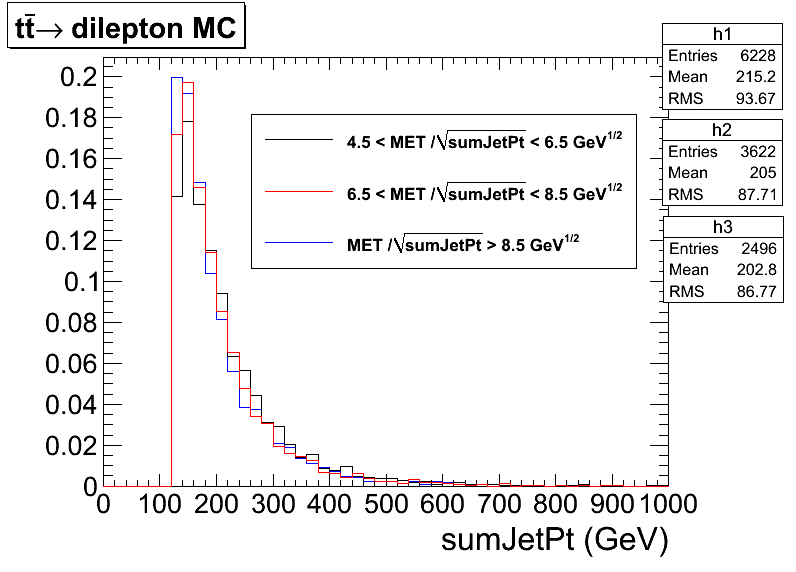
\includegraphics[width=0.75\linewidth]{uncor.png}
\caption{\label{fig:uncor}\protect Distributions of SumJetPt 
in MC $t\bar{t}$ events for different intervals of 
MET$/\sqrt{\rm SumJetPt}$. h1, h2, and h3 refer to the MET$/\sqrt{\rm SumJetPt}$
intervals 4.5-6.5, 6.5-8.5 and $>$8.5, respectively. }
\end{center}
\end{figure}

\begin{figure}[tb]
\begin{center}
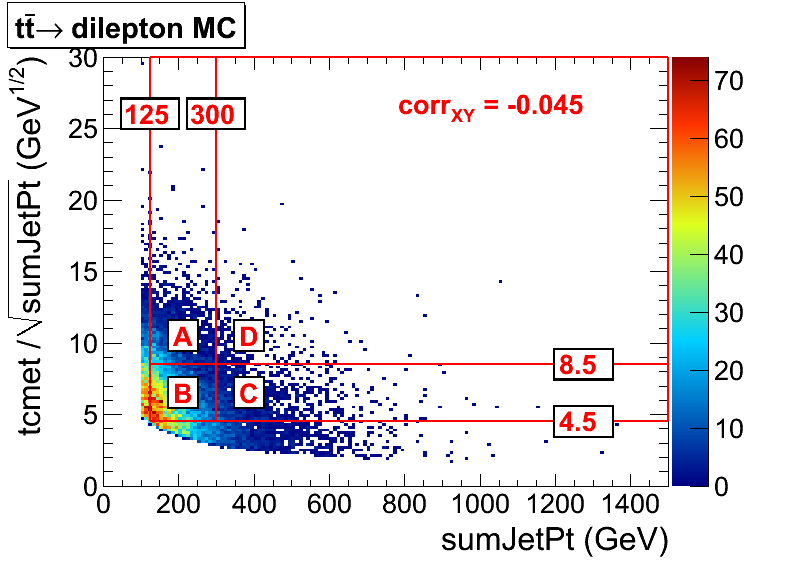
\includegraphics[width=0.75\linewidth]{ttdil_uncor_38X.png}
\caption{\label{fig:abcdMC}\protect Distributions of MET$/\sqrt{\rm SumJetPt}$ vs. 
SumJetPt for SM Monte Carlo.  Here we also show our choice of ABCD regions. The correlation coefficient
${\rm corr_{XY}}$ is computed for events falling in the ABCD regions.}
\end{center}
\end{figure}


Our choice of ABCD regions is shown in Figure~\ref{fig:abcdMC}.
The signal region is region D.  The expected number of events 
in the four regions for the SM Monte Carlo, as well as the background 
prediction A $\times$ C / B are given in Table~\ref{tab:abcdMC} for an integrated
luminosity of 34.0 pb$^{-1}$. In Table~\ref{tab:abcdsyst}, we test the stability of
observed/predicted with respect to variations in the ABCD boundaries. 
Based on the results in Tables~\ref{tab:abcdMC} and~\ref{tab:abcdsyst}, we assess
a systematic uncertainty of 20\% on the prediction of the ABCD method.

%As shown in Table~\ref{tab:abcdsyst}, we assess systematic uncertainties
%by varying the boundaries by an amount consistent with the hadronic energy scale uncertainty,
%which we take as $\pm$5\% for SumJetPt and $\pm$2.5\% for MET/$\sqrt{\rm SumJetPt}$, since the
%uncertainty on this quantity partially cancels due to the fact that it is a ratio of correlated
%quantities. Based on these studies we assess a correction factor $k_{ABCD} = 1.2 \pm 0.2$ to the
%predicted yield using the ABCD method.


%{\color{red} Avi wants some statement about stability 
%wrt changes in regions.  I am not sure that we have done it and 
%I am not sure it is necessary (Claudio).}

\begin{table}[ht]
\begin{center}
\caption{\label{tab:abcdMC} Expected SM Monte Carlo yields for 
34.0~pb$^{-1}$ in the ABCD regions, as well as the predicted yield in
the signal region given by A $\times$ C / B. Here `SM other' is the sum
of non-dileptonic $t\bar{t}$ decays, $W^{\pm}$+jets, $W^+W^-$, 
$W^{\pm}Z^0$, $Z^0Z^0$ and single top.}
\begin{tabular}{lccccc}
%%%official json v3, 38X MC (D6T ttbar and DY)
\hline
              sample                     &                   A   &                   B   &                   C   &                   D   &                PRED  \\
\hline
$t\bar{t}\rightarrow \ell^{+}\ell^{-}$   &   8.44  $\pm$  0.18   &  32.83  $\pm$  0.35   &   4.78  $\pm$  0.14   &   1.07  $\pm$  0.06   &   1.23  $\pm$  0.05  \\
$Z^0 \rightarrow \ell^{+}\ell^{-}$       &   0.17  $\pm$  0.08   &   1.18  $\pm$  0.22   &   0.04  $\pm$  0.04   &   0.12  $\pm$  0.07   &   0.01  $\pm$  0.01  \\
            SM other                     &   0.53  $\pm$  0.03   &   2.26  $\pm$  0.11   &   0.23  $\pm$  0.03   &   0.07  $\pm$  0.01   &   0.05  $\pm$  0.01  \\
\hline
         total SM MC                     &   9.14  $\pm$  0.20   &  36.26  $\pm$  0.43   &   5.05  $\pm$  0.14   &   1.27  $\pm$  0.10   &   1.27  $\pm$  0.05  \\
\hline
\end{tabular}
\end{center}
\end{table}



\begin{table}[ht]
\begin{center}
\caption{\label{tab:abcdsyst} 
Results of the systematic study of the ABCD method by varying the boundaries
between the ABCD regions shown in Fig.~\ref{fig:abcdMC}. Here $x_1$ is the lower SumJetPt boundary and 
$x_2$ is the boundary separating regions A and B from C and D, their nominal values are 125 and 300~GeV,
respectively. $y_1$ is the lower MET/$\sqrt{\rm SumJetPt}$ boundary and 
$y_2$ is the boundary separating regions B and C from A and D, their nominal values are 4.5 and 8.5~GeV$^{1/2}$,
respectively.}
\begin{tabular}{cccc|c}
\hline
$x_1$   &   $x_2$ & $y_1$   &   $y_2$ & Observed/Predicted \\
\hline

nominal & nominal & nominal & nominal & $1.00 \pm 0.08$    \\

+5\%    & +5\%    & +2.5\%  & +2.5\%  & $1.08 \pm 0.11$    \\

+5\%    & +5\%    & nominal & nominal & $1.04 \pm 0.10$    \\

nominal & nominal & +2.5\%  & +2.5\%  & $1.03 \pm 0.09$    \\

nominal & +5\%    & nominal & +2.5\%  & $1.05 \pm 0.10$    \\

nominal & -5\%    & nominal & -2.5\%  & $0.95 \pm 0.07$    \\

-5\%    & -5\%    & +2.5\%  & +2.5\%  & $1.00 \pm 0.08$    \\

+5\%    & +5\%    & -2.5\%  & -2.5\%  & $0.98 \pm 0.09$    \\
\hline
\end{tabular}
\end{center}
\end{table}


\clearpage

\subsection{Dilepton $P_T$ method}
\label{sec:victory}
This method is based on a suggestion by V. Pavlunin\cite{ref:victory},
and was investigated by our group in 2009\cite{ref:ourvictory}.
The idea is that in dilepton $t\bar{t}$ events the lepton and neutrinos
from $W$ decays have the same $P_T$ spectrum (modulo $W$ polarization 
effects).  One can then use the observed 
$P_T(\ell\ell)$ distribution to model the sum of neutrino $P_T$'s which 
is identified with the \met.

Then, in order to predict the $t\bar{t} \to$ dilepton contribution to a 
selection with \met$+$X, one applies a cut on $P_T(\ell\ell)+$X instead.
In practice one has to rescale the result of the $P_T(\ell\ell)+$X selection
to account for the fact that any dilepton selection must include a 
moderate \met cut in order to reduce Drell Yan backgrounds.  This 
is discussed in Section 5.3 of Reference~\cite{ref:ourvictory}; for a \met
cut of 50 GeV, the rescaling factor is obtained from the MC as

\newcommand{\ptll} {\ensuremath{P_T(\ell\ell)}}
\begin{center}
$ K = \frac{\int_0^{\infty} {\cal N}(\ptll)~~d\ptll~}{\int_{50}^{\infty} {\cal N}(\ptll)~~d\ptll~} = 1.5$
\end{center}


%%%TO BE REPLACED
%Given the integrated luminosity of the
%present dataset, the determination of $K$ in data is severely statistics
%limited.  Thus, we take $K$ from $t\bar{t}$ Monte Carlo as 

%\begin{center}
%$ K_{MC} = \frac{\int_0^{\infty} {\cal N}(\met)~~d\met~}{\int_{50}^{\infty} {\cal N}(\met)~~d\met~}$
%\end{center}

%\noindent {\color{red} For the 11 pb result we have used $K$ from data.}


\begin{figure}[bht]
\begin{center}
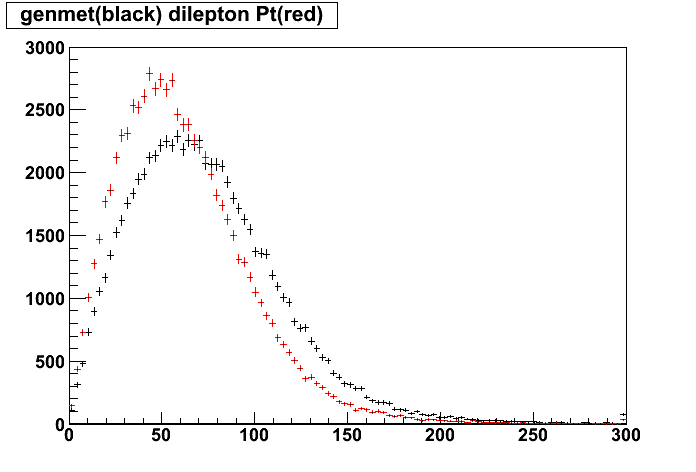
\includegraphics[width=0.75\linewidth]{genvictory_Dec13.png}
\caption{\label{fig:genvictory}\protect Distributions $P_T(\ell \ell)$
and $P_T(\nu \nu)$ (aka {\it genmet})
in $t\bar{t} \to$ dilepton Monte Carlo at the 
generator level.  Events with $W \to \tau \to \ell$ are not included.
No kinematical requirements have been made.} 
\end{center}
\end{figure}


There are several effects that spoil the correspondance between \met and
$P_T(\ell\ell)$: 
\begin{itemize}
\item $Ws$ in top events are polarized.  Neutrinos are emitted preferentially
parallel to the $W$ velocity while charged leptons are emitted prefertially
anti-parallel. Thus the $P_T(\nu\nu)$ distribution is harder
than the $P_T(\ell\ell)$ distribution for top dilepton events.
This turns out to be the dominant effect and it is illustrated in 
Figure~\ref{fig:genvictory}.
\item The lepton selections results in $P_T$ and $\eta$ cuts on the individual
leptons that have no simple correspondance to the neutrino requirements.
\item Similarly, the \met$>$50 GeV cut introduces an asymmetry between leptons and
neutrinos which is only partially compensated by the $K$ factor above.
\item The \met resolution is much worse than the dilepton $P_T$ resolution.
When convoluted with a falling spectrum in the tails of \met, this results
in a harder spectrum for \met than the original $P_T(\nu\nu)$.
\item The \met response in CMS is not exactly 1.  This causes a distortion
in the \met distribution that is not present in the $P_T(\ell\ell)$ distribution.
\item The $t\bar{t} \to$ dilepton signal includes contributions from 
$W \to \tau \to \ell$.  For these events the arguments about the equivalence 
of $P_T(\ell\ell)$ and $P_T(\nu\nu)$ do not apply.
\item A dilepton selection will include SM events from non $t\bar{t}$ 
sources.  These events can affect the background prediction.  Particularly 
dangerous are high $P_T$ Drell Yan events that barely pass the \met$>$ 50 
GeV selection.  They will tend to push the data-driven background prediction up.
Therefore we estimate the number of DY events entering the background prediction
using the $R_{out/in}$ method as described in Sec.~\ref{sec:othBG}.
\end{itemize}

We have studied these effects in SM Monte Carlo, using a mixture of generator and
reconstruction level studies, putting the various effects in one at a time.
For each configuration, we apply the data-driven method and report as figure
of merit the ratio of observed and predicted events in the signal region.
The figure of merit is calculated as follows
\begin{itemize}
\item We construct \met/$\sqrt{{\rm sumJetPt}}$ 
and $P_T(\ell \ell)/\sqrt{{\rm sumJetPt}}$ (rescaled by the factor $K$ defined
above) distributions.  
\item The distributions are constructed using either
GEN or RECO, and including or excluding various effects ({\em e.g.:} 
$t \to W \to \tau \to \ell$).  
\item In all cases the $N_{jets} \ge 2$ and 
sumJetPt $>$ 300 GeV requirements are applied.
\item ``observed events'' is the integral of the \met/$\sqrt{{\rm sumJetPt}}$ distribution
above 8.5.
\item ``predicted events'' is the integral of the $P_T(\ell \ell)/\sqrt{{\rm sumJetPt}}$ distribution
above 8.5.
\end{itemize}
The results are summarized in Table~\ref{tab:victorybad}.  Distributions corresponding to 
lines 4 and 5 of Table~\ref{tab:victorybad} are shown in Figure~\ref{fig:victorybad}.

\begin{table}[htb]
\begin{center}
\caption{\label{tab:victorybad} 
Test of the data driven method in Monte Carlo 
under different assumptions, evaluated using Spring10 MC.  See text for details.}
\begin{tabular}{|l|c|c|c|c|c|c|c|c|}
\hline
& True $t\bar{t}$ dilepton & $t\to W\to\tau$& other SM & GEN or  & Lepton $P_T$    & Z veto & \met $>$ 50& obs/pred \\
& included                 & included       & included & RECOSIM & and $\eta$ cuts &        &            &       \\ \hline
1&Y                        &     N          &   N      &  GEN    &   N             &   N    & N          & 1.90  \\
2&Y                        &     N          &   N      &  GEN    &   Y             &   N    & N          & 1.64  \\
3&Y                        &     N          &   N      &  GEN    &   Y             &   Y    & N          & 1.59  \\
4&Y                        &     N          &   N      &  GEN    &   Y             &   Y    & Y          & 1.55  \\
5&Y                        &     N          &   N      & RECOSIM &   Y             &   Y    & Y          & 1.51  \\
6&Y                        &     Y          &   N      & RECOSIM &   Y             &   Y    & Y          & 1.58  \\
7&Y                        &     Y          &   Y      & RECOSIM &   Y             &   Y    & Y          & 1.38  \\
\hline
\end{tabular}
\end{center}
\end{table}


\begin{figure}[bht]
\begin{center}
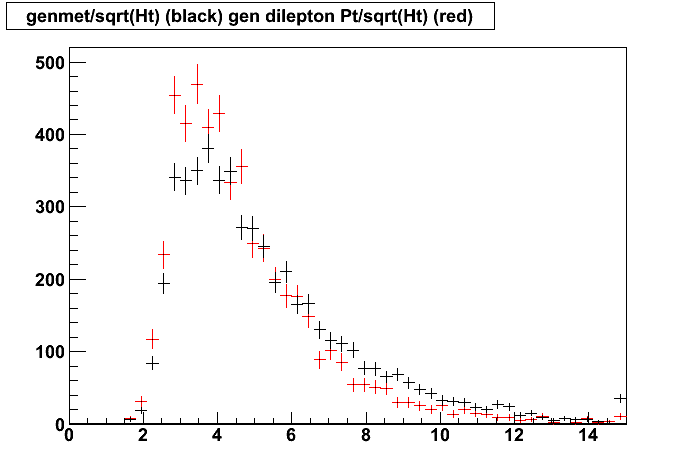
\includegraphics[width=0.48\linewidth]{genvictory_sqrtHt_Dec13.png}
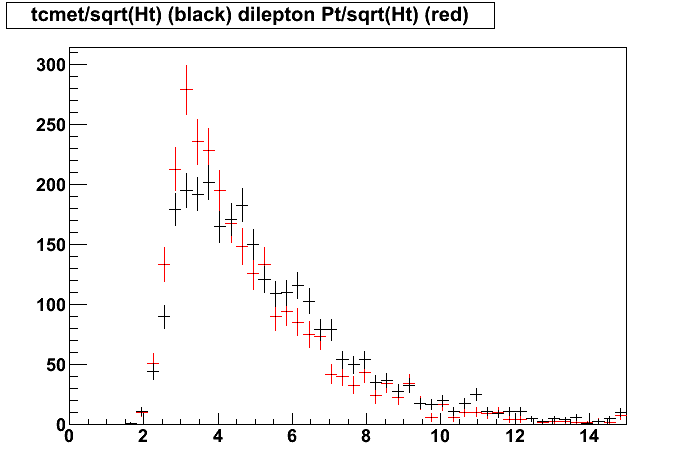
\includegraphics[width=0.48\linewidth]{victory_Dec13.png}
\caption{\label{fig:victorybad}\protect Distributions 
of MET/$\sqrt{{\rm sumJetPt}}$ (black) and $P_T(\ell \ell)/\sqrt{{\rm sumJetPt}}$ 
(red) in $t\bar{t} \to$ dilepton Monte Carlo
after lepton kinematical cuts, $N_{jets} \ge 2$, and 
sumJetPt $>$ 300 GeV.  The left (right) plot is at the GEN (RECO) level 
and corresponds to line 4 (5) of Table~\ref{tab:victorybad}.}
\end{center}
\end{figure}



\begin{table}[htb]
\begin{center}
\caption{\label{tab:victorysyst} 
Summary of variations in $K_C$ due to the MET scale and resolution uncertainty, and to backgrounds other than $t\bar{t} \to$~dilepton. 
In the first table, `up' and `down' refer to shifting the hadronic energy scale up and down by 5\%. In the second table, the quoted value 
refers to the amount of additional smearing of the MET, as discussed in the text. In the third table, the normalization of all backgrounds
other than $t\bar{t} \to$~dilepton is varied. }
\begin{tabular}{ lcccc }
\hline
       MET scale  &      Predicted       &       Observed       &       Obs/pred       \\
\hline
        nominal   &  0.92 $ \pm $ 0.09   &  1.27 $ \pm $ 0.10   &   1.39 $ \pm $ 0.18  \\
            up    &  0.90 $ \pm $ 0.09   &  1.58 $ \pm $ 0.10   &   1.75 $ \pm $ 0.21  \\
          down    &  0.70 $ \pm $ 0.06   &  0.96 $ \pm $ 0.09   &   1.37 $ \pm $ 0.18  \\
\hline
   MET smearing   &      Predicted       &       Observed       &       Obs/pred       \\
\hline
        nominal   &  0.92 $ \pm $ 0.09   &  1.27 $ \pm $ 0.10   &   1.39 $ \pm $ 0.18  \\
           10\%   &  0.88 $ \pm $ 0.09   &  1.28 $ \pm $ 0.10   &   1.47 $ \pm $ 0.19  \\
           20\%   &  0.87 $ \pm $ 0.09   &  1.26 $ \pm $ 0.10   &   1.44 $ \pm $ 0.19  \\
           30\%   &  1.03 $ \pm $ 0.17   &  1.33 $ \pm $ 0.10   &   1.29 $ \pm $ 0.23  \\
           40\%   &  0.88 $ \pm $ 0.09   &  1.36 $ \pm $ 0.10   &   1.55 $ \pm $ 0.20  \\
           50\%   &  0.80 $ \pm $ 0.07   &  1.39 $ \pm $ 0.10   &   1.73 $ \pm $ 0.19  \\
\hline
  non-$t\bar{t} \to$~dilepton bkg   &       Predicted   &           Observed   &           Obs/pred   \\ 
\hline
   ttdil only                       &   0.79 $ \pm $ 0.07   &   1.07 $ \pm $ 0.06   &   1.36 $ \pm $ 0.14   \\
   nominal                          &   0.92 $ \pm $ 0.09   &   1.27 $ \pm $ 0.10   &   1.39 $ \pm $ 0.18   \\
   double non-ttdil yield           &   1.04 $ \pm $ 0.15   &   1.47 $ \pm $ 0.16   &   1.40 $ \pm $ 0.25   \\
\hline
\end{tabular}
\end{center}
\end{table}

The largest discrepancy between prediction and observation occurs on the first 
line of Table~\ref{tab:victorybad}, {\em i.e.}, at the generator level with no
cuts.  We have verified that this effect is due to the polarization of
the $W$ (we remove the polarization by reweighting the events and we get
good agreement between prediction and observation).  The kinematical 
requirements (lines 2,3,4) compensate somewhat for the effect of W polarization. 
Going from GEN to RECOSIM, the change in observed/predicted is small.  
% We have tracked this down to the fact that tcMET underestimates the true \met
% by $\approx 4\%$\footnote{We find that observed/predicted changes by roughly 0.1
%for each 1.5\% change in \met response.}.  
Finally, contamination from non $t\bar{t}$
events can have a significant impact on the BG prediction.  
%The changes between 
%lines 6 and 7 of Table~\ref{tab:victorybad} is driven by 3
%Drell Yan events that pass the \met selection in Monte Carlo (thus the effect
%is statistically not well quantified).

An additional source of concern is that the CMS Madgraph $t\bar{t}$ MC does
not include effects of spin correlations between the two top quarks.  
We have studied this effect at the generator level using Alpgen.  We find
that the bias is (at most) at the few percent level.

Based on the results of Table~\ref{tab:victorysyst}, we conclude that the 
naive data-driven background estimate based on $P_T{(\ell\ell)}$ needs to 
be corrected by a factor of $ K_C = 1.4 \pm 0.2({\rm stat})$.

The dominant sources of systematic uncertainty in $K_C$ are due to non-$t\bar{t} \to$~dilepton backgrounds,
and the MET scale and resolution uncertainties, as summarized in Table~\ref{tab:victorysyst}. 
The impact of non-$t\bar{t}$-dilepton background is assessed
by varying the yield of all backgrounds except for $t\bar{t} \to$~dilepton. 
The uncertainty is assessed as the larger of the differences between the nominal $K_C$ value and the values
obtained using only $t\bar{t} \to$~dilepton MC and obtained by doubling the non $t\bar{t} \to$~dilepton component,
giving an uncertainty of $0.03$.

The uncertainty in $K_C$ due to the MET scale uncertainty is assessed by varying the hadronic energy scale using
the same method as in~\cite{ref:top}, giving an uncertainty of 0.36. 
We also assess the impact of the MET resolution 
uncertainty on $K_C$ by applying a random smearing to the MET. For each event, we determine the expected MET resolution 
based on the sumJetPt, and smear the MET to simulate an increase in the resolution of 10\%, 20\%, 30\%, 40\% and 50\%. 
The results show that $K_C$ does not depend strongly on the MET resolution and we therefore do not assess any uncertainty.

Incorporating all the statistical and systematic uncertainties we find $K_C = 1.4 \pm 0.4$.

\subsection{Signal Contamination}
\label{sec:sigcont}

All data-driven methods are in principle subject to signal contaminations
in the control regions, and the methods described in 
Sections~\ref{sec:abcd} and~\ref{sec:victory} are not exceptions.
Signal contamination tends to dilute the significance of a signal
present in the data by inflating the background prediction.

It is hard to quantify how important these effects are because we 
do not know what signal may be hiding in the data.  Having two
independent methods (in addition to Monte Carlo ``dead-reckoning'')
adds redundancy because signal contamination can have different effects
in the different control regions for the two methods.
For example, in the extreme case of a
new physics signal 
with $P_T(\ell \ell) = \met$, an excess of events would be seen 
in the ABCD method but not in the $P_T(\ell \ell)$ method.


The LM points are benchmarks for SUSY analyses at CMS.  The effects
of signal contaminations for a couple such points are summarized
in Table~\ref{tab:sigcont}. Signal contamination is definitely an important
effect for these two LM points, but it does not totally hide the
presence of the signal.


\begin{table}[htb]
\begin{center}
\caption{\label{tab:sigcont} Effects of signal contamination 
for the two data-driven background estimates. The three columns give
the expected yield in the signal region and the background estimates
using the ABCD and $P_T(\ell \ell)$ methods. Results are normalized to 34.0~pb$^{-1}$.}
\begin{tabular}{lccc}
\hline
            &      Yield      &      ABCD    & $P_T(\ell \ell)$  \\
\hline
SM only     &       1.3      &      1.3    &       0.9        \\
SM + LM0    &       9.9      &      6.1    &       2.4        \\
SM + LM1    &       4.8      &      1.8    &       1.6        \\
%SM only     &       1.27      &      1.27    &       0.92        \\
%SM + LM0    &       7.39      &      4.38    &       1.93        \\
%SM + LM1    &       3.77      &      1.62    &       1.41        \\
\hline
\end{tabular}
\end{center}
\end{table}

